%%%%%%%%%%%%%%%%%%%%%%%%%%%%%%%%%%%%%%%%%
% Presentation Template
% LaTeX Template
% Version 1.0 (2023-02-08)
%
% This template was adapted by:
% Jonathan Decker (jonathan.decker@uni-goettingen.de)
% From a template made by:
% Julian Kunkel (julian.kunkel@gwdg.de)
%
%%%%%%%%%%%%%%%%%%%%%%%%%%%%%%%%%%%%%%%%%
\documentclass[compress,aspectratio=169]{beamer}

% make sure the theme file is on this path
\usepackage{./assets/beamerthemeGoettingen}
\usetikzlibrary{graphs}
\usetikzlibrary {graphs.standard}

\addbibresource{presentation/ref.bib}
\graphicspath{{./}{./assets/}}

% --- document configuration ---
\newcommand{\mytitle}{Rusty Parallel Traveling Salesman Problem Solver}
% Leave empty for no subtitle
\newcommand{\mysubtitle}{walky walky}
\newcommand{\myauthor}{Lars Quentin, Johann Carl Meyer, Dr. Artur Wachtel}
\newcommand{\myauthorurl}{https://github.com/lquenti/walky}
\newcommand{\myvenue}{Practical Course on High-Performance Computing}
% For example, use \today
\newcommand{\mydate}{03.07.2023}
% For example, Institute for Computer Science / GWDG
\newcommand{\myinstitute}{Institute for Computer Science}

\configuretitlepage


\begin{document}

\begin{frame}[plain]
	\titlepage
\end{frame}

\begin{frame}[t]{Table of contents}
  \tableofcontents[subsectionstyle=hide/hide]
\end{frame}

% --- slides begin ---

\section{Introduction}
% This part is to be filled by Johann

% Feel free to change the amount of slides, this is just meant as a starting point

\begin{frame}{Goals}
  \begin{enumerate}
    \item Develop a CLI tool compatible with current state-of-the-art research
    \pause
    \item Performance and Efficiency
      \begin{itemize}
        \item Create a blazingly fast software package
        \item Provide a 100\% pure Rust alternative to classical solvers
        \item Support both shared and distributed memory parallelization
        \item Achieve full documentation coverage
        \item Achieve high unit test coverage
      \end{itemize}
  \end{enumerate}
\end{frame}
\begin{frame}{Goals (cont.)}
  \begin{enumerate}
      \setcounter{enumi}{2}
    \item Exact Solving
      \begin{itemize}
        \item Implement a simple, exact solver for the TSP
        \item Offer several optimized versions
        \item Create a shared memory parallelized verion
        \item Develop a distributed memory, MPI-based parallelized solver
      \end{itemize}
      \pause
    \item Approximation Tactics
      \begin{itemize}
        \item Include a trivial, easy to parallelize tactic and
        \item A sophisticated, state of the art tactic
        \item For both:
          \begin{itemize}
            \item Provide a shared memory parallelized solver
            \item Provide a distributed memory, MPI based parallelized solver
          \end{itemize}
      \end{itemize}
      \pause
    \item Lower Bound Calculation for TSP
      \begin{itemize}
        \item Provide a sequential implementation
        \item Develop a parallelized implementation using MPI
      \end{itemize}
  \end{enumerate}
\end{frame}

\begin{frame}{Organizational Remark}
  Targeted Credits for this course:
  \begin{itemize}
    \item Lars: 9C
    \item Johann: 6C
  \end{itemize}
~\\
  See also \url{https://hps.vi4io.org/_media/teaching/summer_term_2023/pchpc/pchpcassignment.pdf}
  for expected work depending on the targeted credits.
\end{frame}

% Or any other kind of information
\begin{frame}{Travelling Salesman Problem Definition}
\begin{minipage}{0.45\textwidth}
  \includegraphics[width=0.8\textwidth]{TSP_Deutschland_3}
  \tiny

  user "Kapitän Nemo" \url{https://commons.wikimedia.org/w/index.php?curid=5584283}
\end{minipage}
\begin{minipage}{0.45\textwidth}

"Given a list of cities and the distances between each pair of cities, what is the shortest possible route that visits each city exactly once and returns to the origin city?"
\cite{song_solving_2021}
\end{minipage}
\end{frame}

\begin{frame}{Travelling Salesman Problem Definition}
  \begin{itemize}
    \item input graph
      \begin{itemize}
        \item weighted, non-negative
        \item undirected
        \item complete (fully connected)
      \end{itemize}

    \pause
    \item output restrictions:
      \begin{itemize}
        \item tour (cycle that visits every vertex)
        \item use any edge \emph{at most} one time
      \end{itemize}
    \pause
    \item problem: find a legal output that has minimal (cumulative) edge weight
  \end{itemize}
\end{frame}

\begin{frame}{Why is TSP interesting?}
  \begin{itemize}
    \item well studied
    \item NP-complete $\rightarrow$ ressource intensive
    \item intuitive to understand
    \pause
    \item practical applications (see \href{https://en.wikipedia.org/wiki/Concorde_TSP_Solver}{Concorde TSP Solver})
  \end{itemize}
  % https://upload.wikimedia.org/wikipedia/commons/c/c4/TSP_Deutschland_3.png
\end{frame}

\begin{frame}{Our Implementation}
  \begin{itemize}
    \item Publicly available on GitHub
    \item can be found on at \url{https://crates.io/crates/walky/}
    \item licensed under the MIT open source license
  \end{itemize}
\end{frame}

%\begin{frame}{MST}
%\end{frame}


\section{Exact Solving}
% This part is to be filled by Lars

\begin{frame}{Na\"ive Approach}
  \begin{columns}
    \begin{column}{0.5\textwidth}
      \begin{itemize}
        \item Test out all possible paths
        \item Keep the shortest one
        \item Using Fast iterative enumeration algorithm \cite{nayuki_next_nodate}
        \item First Optimization: Fixate the first element!
        \item Complexity: $\Theta(n!)$
      \end{itemize}
    \end{column}
    \pause
    \begin{column}{0.5\textwidth}
      \begin{figure}
      \footnotesize\inputminted[xleftmargin=1em,fontsize=\tiny,linenos]{rust}{./assets/02_first_impl.rs}
      \end{figure}
    \end{column}
  \end{columns}
\end{frame}

\begin{frame}{Cache Prefix Sums}
  \begin{columns}
    \begin{column}{0.5\textwidth}
      \begin{itemize}
        \item After every path, we compute the tour
        \item Reuse partial computations
        \item While enumerating, keep prefix as long as possible
          \begin{itemize}
            \item \textbf{Recursive enumeration!}
          \end{itemize}
      \end{itemize}
    \end{column}
    \pause
    \begin{column}{0.5\textwidth}
      \begin{figure}
      \footnotesize\inputminted[xleftmargin=1em,fontsize=\small,linenos]{python}{./assets/02_recenum.py}
      \end{figure}
    \end{column}
  \end{columns}
  \pause
  \begin{center}
    {\Large But do we \textit{actually} have to look at every solution?}
  \end{center}
\end{frame}

\begin{frame}{Pruning}
  \vspace*{-0.5cm}
  \begin{columns}
    \begin{column}{0.5\textwidth}
      \begin{block}{V1: Stop what doesn't work!}
        \begin{itemize}
          \item Use the partial sum
          \item Lower bound: Previous best
          \item {\small\texttt{if (partial\_sum <= prev\_best) rec\_enum(...)}}
        \end{itemize}
      \end{block}
      \pause
      \begin{block}{V2: Nearest Neighbour (NN)}
        \begin{itemize}
          \item prune if \texttt{(partial\_sum + lower\_bound)} of remaining vertices
          \item Lower bound:
            \begin{itemize}
              \item Connect every vertex to the nearest one!
            \end{itemize}
        \end{itemize}
      \end{block}
    \end{column}
    \pause
    \begin{column}{0.5\textwidth}
      \includegraphics[width=\textwidth]{./assets/nn.png}
    \end{column}
  \end{columns}
\end{frame}

\begin{frame}{Pruning (cont.)}
  \vspace*{-0.5cm}
  \begin{columns}
    \begin{column}{0.5\textwidth}
      \begin{block}{V3: Minimal Spanning Tree (MST)}
        \begin{itemize}
          \item Same idea
          \item Use Minimal Spanning Tree of remaining vertices
          \item $NN < MST < TSP$
        \end{itemize}
      \end{block}
      \pause
      \begin{block}{V4: Caching}
        \begin{itemize}
          \item Cache the MST in a HashMap
          \item Using a non-cryptographic HashMap
        \end{itemize}
      \end{block}
    \end{column}
    \pause
    \begin{column}{0.5\textwidth}
      \includegraphics[width=\textwidth]{./assets/mst.png}
    \end{column}
  \end{columns}
\end{frame}

\begin{frame}{Benchmarking Results}
  \vspace{-0.25cm}
  \begin{figure}
    \includegraphics[width=\linewidth,height=.9\textheight,keepaspectratio]{./assets/v0.pdf}
  \end{figure}
\end{frame}
\begin{frame}{Benchmarking Results}
  \vspace{-0.25cm}
  \begin{figure}
    \includegraphics[width=\linewidth,height=.9\textheight,keepaspectratio]{./assets/v1.pdf}
  \end{figure}
\end{frame}
\begin{frame}{Benchmarking Results}
  \vspace{-0.25cm}
  \begin{figure}
    \includegraphics[width=\linewidth,height=.9\textheight,keepaspectratio]{./assets/v2.pdf}
  \end{figure}
\end{frame}
\begin{frame}{Benchmarking Results}
  \vspace{-0.25cm}
  \begin{figure}
    \includegraphics[width=\linewidth,height=.9\textheight,keepaspectratio]{./assets/v3.pdf}
  \end{figure}
\end{frame}
\begin{frame}{Benchmarking Results}
  \vspace{-0.25cm}
  \begin{figure}
    \includegraphics[width=\linewidth,height=.9\textheight,keepaspectratio]{./assets/v4.pdf}
  \end{figure}
\end{frame}
\begin{frame}{Benchmarking Results}
  \vspace{-0.25cm}
  \begin{figure}
    \includegraphics[width=\linewidth,height=.9\textheight,keepaspectratio]{./assets/v5.pdf}
  \end{figure}
\end{frame}
\begin{frame}{Benchmarking Results}
  \vspace{-0.25cm}
  \begin{figure}
    \includegraphics[width=\linewidth,height=.9\textheight,keepaspectratio]{./assets/v6.pdf}
  \end{figure}
\end{frame}

\begin{frame}{Threading}
  \begin{block}{Algorithm}
    \begin{enumerate}
        \pause
      \item Spawn $n$ threads
        \pause
      \item Divide the prefix space locally, $i$-th thread gets $i$-th chunk
        \pause
      \item Compute next prefix (with MST lower bound)
        \pause
      \item Update local optimum shared with all threads
        \pause
      \item \texttt{GOTO 3} until done with chunk
    \end{enumerate}
  \end{block}
\end{frame}
\begin{frame}{Benchmarking Results}
  \vspace{-0.25cm}
  \begin{figure}
    \includegraphics[width=\linewidth,height=.9\textheight,keepaspectratio]{./assets/v7.pdf}
  \end{figure}
\end{frame}

\begin{frame}{MPI}
  \begin{block}{Computation}
  \begin{itemize}
    \item One coordinator, $n-1$ worker
      \pause
    \item Prefix chunk division like threaded
      \pause
    \item After each prefix, the worker reports current best \textbf{cost} to coordinator
      \pause
    \item Coordinator answers with global best \textbf{cost}
      \begin{itemize}
        \item Tightest possible bound for pruning
      \end{itemize}
      \pause
    \item At the end, worker tells coordinator that its done and waits at barrier
      \pause
    \item After all are done, coordinator joins the barrier
  \end{itemize}
  \end{block}
\end{frame}

\begin{frame}{MPI (cont.)}
  \begin{block}{Joining the local optima}
  \begin{itemize}
      \pause
    \item After all are done, the coordinator broadcasts
      \begin{itemize}
        \item which rank won
        \item and the minimal cost
      \end{itemize}
      \pause
    \item That rank then broadcasts \textbf{the full path}
      \begin{itemize}
        \item This is an traffic efficiency optimization!
      \end{itemize}
  \end{itemize}
  \pause
  Now every process knows the best cost and path.
  \end{block}
\end{frame}

\begin{frame}{Benchmarks}
  \vspace{-0.25cm}
  \begin{figure}
    \includegraphics[width=\linewidth,height=.9\textheight,keepaspectratio]{./assets/exact-mpi.pdf}
  \end{figure}
\end{frame}


\section{Approximation}
% This part is to be filled by Lars

\begin{frame}{Nearest Neighbour}
  \begin{block}{Single Nearest Neighbour}
    \begin{enumerate}
      \item Start at a random node
      \item Check distances to all unvisited nodes
      \item Go to the one with the shortest distance
      \item \texttt{GOTO 2} until all nodes are visited
    \end{enumerate}
  \end{block}
  \pause
  \begin{block}{Nearest Neighbour}
    \begin{itemize}
      \item Do Single NN for every starting node
      \item Choose the best
    \end{itemize}
  \end{block}
\end{frame}

\begin{frame}{Nearest Neighbour (cont.)}
      \begin{block}{Single Threaded}
      \footnotesize\inputminted[xleftmargin=1em,fontsize=\large,linenos]{rust}{./assets/03_NN_single.rs}
      \end{block}
\end{frame}

\begin{frame}{Nearest Neighbour (cont.)}
      \begin{block}{Multi Threaded}
        \footnotesize\inputminted[xleftmargin=1em,fontsize=\large,linenos]{rust}{./assets/03_NN_parallel.rs}
      \end{block}
\end{frame}


\begin{frame}{Benchmarks}
  \vspace{-0.25cm}
  \begin{figure}
    \includegraphics[width=\linewidth,height=.9\textheight,keepaspectratio]{../assets/nn-stmt.pdf}
  \end{figure}
\end{frame}

\begin{frame}{Nearest Neighbour: MPI}
  \begin{itemize}
    \item Divide number of nodes into equal chunks
      \pause
    \item Every process computes their chunks
      \pause
    \item \texttt{MPI\_Allreduce} the \textbf{cost} (and keep rank)
      \pause
    \item Winner rank \texttt{MPI\_Bcast} the solution path.
  \end{itemize}
\end{frame}

\begin{frame}{Benchmarks}
  \vspace{-0.25cm}
  \begin{figure}
    \includegraphics[width=\linewidth,height=.9\textheight,keepaspectratio]{../assets/nn-mpi.pdf}
  \end{figure}
\end{frame}

% This part is to be filled by Johann
\subsection{Christofides Algorithm}

\begin{frame}[t]{Christofides Algorithm}
  \begin{itemize}
    \item Assumption: the input graph is metric, i.e. the triangle inequality holds
    \pause
    \item the algorithm goes as following \cite{christofides_worst-case_1976}:
      \begin{enumerate}
        \item calculate the MST
        \pause
        \item calculate a matching in the complete graph of minimum weight, over all vertices, that have odd degree in the MST
          \begin{itemize}
            \item see also next slides
          \pause
            \item parallelization: mostly in this step
          \end{itemize}
        \pause
        \item combine the MST and the matching into one multigraph
        \pause
        \item find an eulerian cycle through the multigraph
        \pause
        \item make the eulerian cycle hamiltonian
      \end{enumerate}
  \end{itemize}
\end{frame}

\begin{frame}[t]{Christofides Algorithm: Where To Find A Matching?}
  Complete input graph with highlighted MST:

  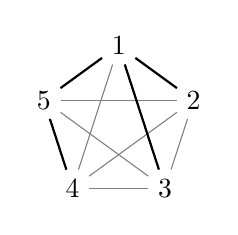
\begin{tikzpicture}
    \graph { subgraph K_n [n=5, clockwise, edges=gray];
      (1) --[thick] (2);
      (1) --[thick] (5);
      (5) --[thick] (4);
      (1) --[thick] (3); };
    
  \end{tikzpicture}

  Vertices with odd degree: $1,2,3,4$. $\hookrightarrow$ Find a matching over these vertices (blue):

  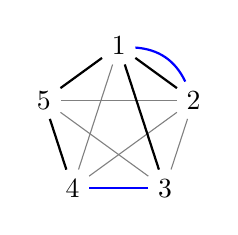
\begin{tikzpicture}
    \graph { subgraph K_n [n=5, clockwise, edges=gray];
      (1) --[thick] (2);
      (1) --[thick] (5);
      (5) --[thick] (4);
      (1) --[thick] (3);
      (4) --[thick, blue] (3);
      (1) --[thick, blue, bend left] (2);
    };
  \end{tikzpicture}

  Note: edge weights are left out for simplicity
\end{frame}

\begin{frame}[t]{Christofides Algorithm: Finding A Matching}
  Finding a minimum cost matching:
  \begin{itemize}
    \item exact solution:
      \begin{itemize}
        \item uses a sophisticated algorithm (the \href{https://en.wikipedia.org/wiki/Blossom_algorithm}{blossom algorithm})
        \item hard to parallelize
        \item slow (uses a lot of HashSets)
      \end{itemize}
      \pause
    \item randomized approximate solution:
      \begin{itemize}
        \item idea: guess a matching and do some randomized improvements.\\Repeat this and take the best matching
        \item easy to implement
        \item easy to parallelize
      \end{itemize}
  \end{itemize}
\end{frame}

\begin{frame}[t]{Christofides Algorithm: Randomly Finding A Matching}
  \vfill
  Finding a matching: the graph is complete \& has even amount of vertices (trivial)

  \begin{enumerate}
    \item Given the list of all vertices $[0,1,2,3,4,5,6,7]$
    \item randomly scramble the list: $[2,1,0,3,7,5,6,4]$
    \item interpret the list as a matching: $[[2,1],[0,3],[7,5],[6,4]]$
  \end{enumerate}
  \vfill
\end{frame}

\begin{frame}[t]{Christofides Algorithm: Improving A Matching Of 4 Vertices}
  \vfill
  Improving a matching on 4 vertices: easy: only 3 cases to consider:
  \vfill

  \hfill
  \begin{tikzpicture}
    \node (1) at (0,1) {1};
    \node (2) at (0,0) {2};
    \node (3) at (1,1) {3};
    \node (4) at (1,0) {4};
    \graph { (1) -- (2); (3) -- (4)  };
  \end{tikzpicture}, \hfill or \hfill
  \begin{tikzpicture}
    \node (1) at (0,1) {1};
    \node (2) at (0,0) {2};
    \node (3) at (1,1) {3};
    \node (4) at (1,0) {4};
    \graph { (1) -- (3); (2) -- (4)  };
  \end{tikzpicture} \hfill or \hfill
  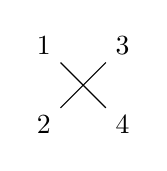
\begin{tikzpicture}
    \node (1) at (0,1) {1};
    \node (2) at (0,0) {2};
    \node (3) at (1,1) {3};
    \node (4) at (1,0) {4};
    \graph { (1) -- (4); (2) -- (3)  };
  \end{tikzpicture}

  \vfill
  Chose the matching with the lowest cost.
  \vfill
\end{frame}

\begin{frame}[t]{Christofides Algorithm: Randomly Improving A Matching}
  \vfill
  Improving a matching:\\
  improve pairs of edges:
  \begin{enumerate}
    \item Given a matching $[[2,1],[0,3],[7,5],[6,4]]$
    \item randomly scramble the list: $[[7,5],[0,3],[2,1],[6,4]]$ \label{itemize:random_edge_scramble}
    \item consider consecutive blocks of two edges: $[7,5],[0,3]$ and $[2,1],[6,4]$
    \item for a block of two edges, consider the other two possible matchings among the four vertices, are they better? Given:
      $[7,5],[0,3]$ consider $[7,0], [5,3]$ and $[7,3], [5,0]$
    \item repeat with step \ref{itemize:random_edge_scramble}
  \end{enumerate}
  \vfill
\end{frame}

\begin{frame}[t]{Christofides Algorithm: Randomly Improving A Matching In Parallel}
  \vfill
  Parallelize the randomized algorithm: do the same thing many times in parallel
  
  \begin{enumerate}
    \item each process: generates a random matching, and randomly improves it
    \item then: pick the best result and return it
  \end{enumerate}
  \vfill
\end{frame}

\begin{frame}[t]{Christofides Algorithm: Benchmarking}
  \vfill
  Christofides algorithm does not benefit from parallelization w.r.t. execution time:
  
  \begin{figure}
    \includegraphics[width=\linewidth,height=0.8\textheight,keepaspectratio]{christofides-stmt.pdf}
  \end{figure}
  \vfill
\end{frame}

\begin{frame}[t]{Christofides Algorithm: Benchmarking}
  \vfill
  Christofides algorithm does slightly benefit w.r.t. solution weight:
  
  \begin{figure}
    \includegraphics[width=\linewidth,height=0.8\textheight,keepaspectratio]{christofides-mpi.pdf}
  \end{figure}
  \vfill
\end{frame}

% This part is to be filled by Johann
\subsection{1-tree lower bound}

\begin{frame}[t]{How To Get A 1-tree Lower Bound?}
  Start with an MST over $n-1$ edges (here vertex $4$ is left out):

  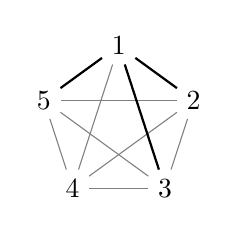
\begin{tikzpicture}
    \graph { subgraph K_n [n=5, clockwise, edges=gray];
      (1) --[thick] (2);
      (1) --[thick] (5);
      (1) --[thick] (3); };
    
  \end{tikzpicture}

  Then add the remaining vertex, and the two edges with lowest cost adjacent to that vertex:

  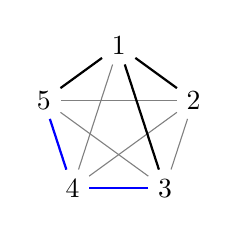
\begin{tikzpicture}
    \graph { subgraph K_n [n=5, clockwise, edges=gray];
      (1) --[thick] (2);
      (1) --[thick] (5);
      (5) --[thick, blue] (4);
      (1) --[thick] (3);
      (4) --[thick, blue] (3);
    };
  \end{tikzpicture}
\end{frame}

\begin{frame}[t]{Lower Bound With 1-tree on TSP}
  \vfill

  \begin{itemize}
    \item any 1-tree weight is a lower bound on the TSP solution \cite{held_traveling-salesman_1970}
    \item $|V|$ 1-trees to check independently
    \item very easy to parallelize
  \end{itemize}

  \vfill
\end{frame}

\begin{frame}[t]{1-tree Lower Bound Benchmarking}
  \vfill
  The 1-tree lower bound benefits from parallelization:
  
  \begin{figure}
    \includegraphics[width=\linewidth,height=0.8\textheight,keepaspectratio]{1-tree-stmt.pdf}
  \end{figure}
  \vfill
\end{frame}

\begin{frame}[t]{1-tree Lower Bound Benchmarking}
  \vfill
  The 1-tree lower bound benefits from parallelization:
  
  \begin{figure}
    \includegraphics[width=\linewidth,height=0.8\textheight,keepaspectratio]{1-tree-mpi.pdf}
  \end{figure}
  \vfill
\end{frame}


\section{Conclusion}
% This part is to be filled by Lars

\begin{frame}{Future Work}
  \begin{block}{Exact Solver: Dynamic Load Distribution}
    \begin{itemize}
      \item Pruning makes the actual work load unpredictable
      \item Instead of dividing chunks, the coordinator gives out work dynamically
      \item Pro: More equal work distribution
      \item Contra: More communication
    \end{itemize}
  \end{block}
  \pause
  \begin{block}{More MPI analysis and performance tuning}
    \begin{itemize}
      \item Especially using Vampir
    \end{itemize}
  \end{block}
\end{frame}

\begin{frame}{Contribution}
\label{pg:lastpage} % Label on last frame to get the page number for footer
  \vspace{-0.25cm}
  \begin{enumerate}
    \item Developed a CLI tool compatible with TSPLIB
      \pause
    \item Provided a software that is
      \begin{itemize}
        \item Blazingly fast
        \item Pure Rust (compatible with C-based MPI flavours)
        \item Supports shared- and distributed memory parallelization
        \item Well documented and thoroughly tested
      \end{itemize}
      \pause
    \item Including an exact solver
      \begin{itemize}
        \item With several pruning-based optimizations
        \item Both shared- and distributed memory parallelized
      \end{itemize}
      \pause
    \item And multiple approximate solvers
      \begin{itemize}
        \item Including the easy to parallelize "Nearest Neighbour" method
        \item Supporting the sophisticated "Christofides" algorithm
        \item Both shared- and distributed memory parallelized
      \end{itemize}
      \pause
    \item Implemented the 1-tree lower bound
      \begin{itemize}
        \item Utilized shared- and distributed memory parallelization
      \end{itemize}
  \end{enumerate}
\end{frame}






\begin{frame}{References}
    % References slide in appendix
    \renewcommand*{\bibfont}{\normalfont\scriptsize}
    \printbibliography[heading=none]
\end{frame}

\end{document}
